\section{Programming in C/C++ - The WiringPi Way}
\label{app:C/C++}
Please note that this guide is by no means meant to serve as a comprehensive reference. Rather, it is included to show what WiringPi offers.

\href{http://wiringpi.com}{WiringPi} is a C library (that can be used in C or C++) developed by Gordon Henderson (\href{https://twitter.com/drogon}{@drogon}). Despite the fact that the library has recently been \href{http://wiringpi.com/wiringpi-deprecated/}{deprecated}, it remains an easy way of interfacing with the Raspberry Pi and its peripherals. 

Documentation for the library can be found here: \href{http://wiringpi.com/}{http://wiringpi.com/}.

\subsection{WiringPi on the CommandLine - gpio utility}
Before jumping in to WiringPi and using it in a C/C++ application, it's useful to note that WiringPi has a command line tool that can be used to control the pins. More information on this can be found \href{http://wiringpi.com/the-gpio-utility/}{here}.


\subsection{Working with WiringPi}
To use WiringPi in your code, you need to include it as you would any library. It generally comes installed on Raspbian, so you can just include it as follows:
\begin{lstlisting}
#include <wiringPi.h>
\end{lstlisting}

You also need to link it when compiling to make use of some of the more advanced functionality. See Section \ref{sec:ToolchainsCompilersMakefiles} to better understand this.
\begin{lstlisting}
-lwiringPi
\end{lstlisting}

You need to specify which board mode you're using. For more information on board modes, see Section \ref{sec:BoardModes}. Board modes are specified when  the library is initialized as shown below. These functions need to be run with root privileges, so make sure to use \verb|sudo ./your_program|. 
\begin{lstlisting}
//Initialises WiringPi and assumes that the calling program is going to be using the wiringPi pin numbering scheme.
wiringPiSetup();

//Initialises WiringPi and allows the calling programs to use the Broadcom GPIO pin numbers directly with no re-mapping.
wiringPiSetupGpio();

//Initialises WiringPi and allows the calling programs to use the physical pin numbers on the P1 connector only.
wiringPiSetupPhys();
\end{lstlisting}

You also need to perform "cleanup" on GPIOs when your application exists. By performing cleanup and resetting all pins to their default modes, you can prevent possible damage to your Raspberry Pi. There is not default cleanup function in WiringPi, so you need to write your own.



\subsection{Core Functions}
This section covers the core functions available in the WiringPi library. Read the documentation, available \href{http://wiringpi.com/reference/core-functions/}{here}.

\begin{itemize}
    \item Set the Pin Mode
        \begin{lstlisting}[gobble = 8]
        void pinMode (int pin, int mode) ;
        \end{lstlisting}
        This sets the mode of a pin to either INPUT, OUTPUT, PWM\_OUTPUT or GPIO\_CLOCK. Note that only wiringPi pin 1 (BCM\_GPIO 18) supports PWM output and only wiringPi pin 7 (BCM\_GPIO 4) supports CLOCK output modes.
    \item Set the Internal Resistors
        \begin{lstlisting}[gobble = 8]
        void pullUpDnControl (int pin, int pud) ;
        \end{lstlisting}
        This sets the pull-up or pull-down resistor mode on the given pin, which should be set as an input. The parameter \verb|pud| can be one of the following:
        \begin{itemize}
            \item \verb|PUD_OFF| - no pull up/down 
            \item \verb|PUD_DOWN| - pull to ground 
            \item \verb|PUD_UP| -  pull to 3.3v 
        \end{itemize}
        The internal pull up/down resistors have a value of roughly 50KΩ on the Raspberry Pi.
    \item Write a Digital Value
        \begin{lstlisting}[gobble = 8]
        void digitalWrite (int pin, int value) ;
        \end{lstlisting}
        Writes the value HIGH or LOW (1 or 0) to the given pin which must have been previously set as an output. WiringPi treats any non-zero number as HIGH, however 0 is the only representation of LOW.
    
    \item Read a Digital Value
        \begin{lstlisting}[gobble = 8]
        int digitalRead (int pin) ;
        \end{lstlisting}
        This function returns the value read at the given pin. It will be HIGH or LOW (1 or 0) depending on the logic level at the pin.
    \end{itemize}

\subsection{Analog}
The Raspberry Pi does not have any analog input pins. You will need to use something like the \href{https://cdn-shop.adafruit.com/datasheets/MCP3008.pdf}{MCP3008} to read analog voltages.

\subsection{PWM}
\subsubsection{Hardware PWM}
Read the documentation \href{http://wiringpi.com/reference/raspberry-pi-specifics/}{here}.
To see which pins support hardware PWM, consult \href{pinout.xyz}{pinout.xyz}.
The following functions are available:
\begin{itemize}
    \item Set the PWM mode
        \begin{lstlisting}[gobble=8]
        pwmSetMode (int mode);
        \end{lstlisting}
        The PWM generator can run in 2 modes – “balanced” and “mark:space”. The mark:space mode is traditional, however the default mode in the Pi is “balanced”. You can switch modes by supplying the parameter: \verb|PWM_MODE_BAL| or \verb|PWM_MODE_MS|.
    \item Set the range register
        \begin{lstlisting}[gobble=8]
        pwmSetRange (unsigned int range) ;
        \end{lstlisting}
        The default is 1024.
    \item Set the divisor register
        \begin{lstlisting}[gobble=8]
        pwmSetClock (int divisor) ;
        \end{lstlisting}
\end{itemize}
\subsubsection{Software PWM}
Read the documentation \href{http://wiringpi.com/reference/software-pwm-library/}{here}.
If you're using PWM and it's not on the PWM pin on the Pi, you must include \verb|softPwm|:
\begin{lstlisting}
#include <softPwm.h>
\end{lstlisting}

When compiling, you will alos need to link the PThreads library:
\begin{lstlisting}
-lpthread
\end{lstlisting}

The following functions are available:
\begin{itemize}
    \item Create a software PWM signal:
        \begin{lstlisting}[gobble=8]
        int softPwmCreate (int pin, int initialValue, int pwmRange) ;
        \end{lstlisting}
        You can use any GPIO pin and the pin numbering will be that of the wiringPiSetup() function you used. Use 100 for the pwmRange, then the value can be anything from 0 (off) to 100 (fully on) for the given pin.

        The return value is 0 for success. Anything else and you should check the global errno variable to see what went wrong.
    \item Create a software PWM signal:
        \begin{lstlisting}[gobble=8]
        void softPwmWrite (int pin, int value) ;
        \end{lstlisting}
        This updates the PWM value on the given pin. The value is checked to be in-range and pins that haven’t previously been initialised via softPwmCreate will be silently ignored.
\end{itemize}

Notes on software PWM:
\begin{itemize}
    \item Each “cycle” of PWM output takes 10mS with the default range value of 100, so trying to change the PWM value more than 100 times a second will be futile.
    \item Each pin activated in softPWM mode uses approximately 0.5% of the CPU.
    \item There is currently no way to disable softPWM on a pin while the program in running.
    \item You need to keep your program running to maintain the PWM output!
\end{itemize}


\subsection{Interrupts} 
Very often it is useful to set up an interrupt, for example to trigger an event when a button is pressed. Callback functions are executed on a different thread. If you have multiple callbacks, know that they will be executed sequentially as only one thread exists for interrupts. Interrupts can be implemented as follows:

\begin{lstlisting}
 int wiringPiISR (int pin, int edgeType,  void (*function)(void)) ;
\end{lstlisting}

An example of how to set up a button connected between ground and pin 23 to be used as an interrupt could be as follows:
\begin{lstlisting}
pinMode(23, INPUT); 
pullUpDnControl(23, PUD_UP);
wiringPiISR(23,INT_EDGE_RISING,&callback_function);
\end{lstlisting}

\subsubsection{Software Debounce}
Deboucing is important to prevent multiple triggers of an interrupt. There are two options, hardware and software debounce. Software debounce in C could be implemented as follows:

\begin{lstlisting}
void callback_function(void){}
    long interruptTime = millis();
	
    if (interruptTime - lastInterruptTime>200){
        // Perform your logic here		
    }
    lastInterruptTime = interruptTime;
}
\end{lstlisting}

\subsection{Communication Protocols}
WiringPi, unlike RPI.GPIO, offers methods for communication. 

\subsubsection{I2C}
Read the documentation at \href{http://wiringpi.com/reference/i2c-library/}{WiringPi I2C}, and be sure to link WiringPi when compiling.

Ensure you enable I2C in \verb|raspi-config|.

Once you connect a device, you can run \verb|$gpio i2cdetect| to determine if a device is detected on the I2C bus. In the example below, there is an electronic compass (GY-271) connected to the Pi.
\begin{figure}[H]
\centering
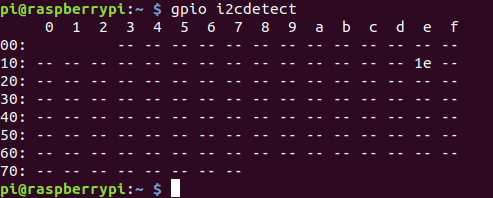
\includegraphics[width=0.7\columnwidth]{Figures/i2cdetect}
\caption{An i2cdetect example}
\end{figure}

To initialize an I2C device, do the following:
\begin{lstlisting}
#include <wiringPiI2C.h>
\end{lstlisting}
And call the function:
\begin{lstlisting}
int wiringPiI2CSetup (int devId) ;
\end{lstlisting}
The function returns a negative 1 if an error occurs. If we want to make use of this functionality, we can write code similar to the following:
\begin{lstlisting}
if (wiringPiI2CSetup (0x1e) == -1) {
    printf("I2C init failed \n");
    return;
}
\end{lstlisting}

\textbf{Note:} For all the following functions, if the return value is negative then an error has happened and you should consult errno.

To read a byte from the I2C device, you can use the following function:
\begin{lstlisting}
int wiringPiI2CReadReg8 (int fd, int reg) ;
\end{lstlisting}

To write a byte to the I2C device:
\begin{lstlisting}
int wiringPiI2CWriteReg8 (int fd, int reg, int data) ;
\end{lstlisting}

Tying all these together, we can create an example. Imagine an I2C device that holds a simple count value, which we want to increase by 1. We can do the following:
\begin{lstlisting}
int i2cdevice = wiringPiI2CSetup (0x1e);
if (i2cdevice == -1) {
    printf("I2C init failed \n");
    return;
}

int value = wiringPiI2CReadReg8(i2cdevice, 0x01);
value = value +1;
wiringPiI2CWriteReg8(i2cdevice, 0x01, value) ;
\end{lstlisting}

\subsubsection{SPI}
Read the documentation at \href{http://wiringpi.com/reference/spi-library/}{WiringPi SPI}, and be sure to link WiringPi when compiling.
Ensure you enable SPI in \verb|raspi-config|. 

To initialize SPI, include the header:
\begin{lstlisting}
#include <wiringPiSPI.h>
\end{lstlisting}
You also need to call the Setup function. \verb|channel| refers to whichever SPI channel you use (0 or 1, based on the pins you use). Speed is the speed in Hz, and is an integer in the range 500,000 through 32,000,000.
\begin{lstlisting}
int wiringPiSPISetup (int channel, int speed) ;
\end{lstlisting}

To write a value through SPI, the following function is used:
\begin{lstlisting}
int wiringPiSPIDataRW (int channel, unsigned char *data, int len) ;
\end{lstlisting}
This performs a simultaneous write/read transaction over the selected SPI bus. \textbf{Data that was in your buffer is overwritten by data returned from the SPI bus.}

Tying this together, we can develop the following example:
\begin{lstlisting}
spidevice = wiringPiSPISetup(0, 1000000) ; // Channel 0 at 1MHz
if (spidevice == -1) {
    printf("SPI init failed \n");
    return;
}

unsigned char data = {0x01, 0x02, 0x03};

wiringPiSPIDataRW(0, data, 3);

printf{"Obtained these values off spidevice:\n"};
for(int i = 0; i < 3; i++){
    printf("%u", data[i]);
}

\end{lstlisting}

\subsection{Timing}
The WiringPi library has some other useful timing functions. Read the documentation \href{http://wiringpi.com/reference/timing/}{here}. These include:
\begin{itemize}
    \item unsigned int millis (void);\\
        This returns a number representing the number of milliseconds since your program called one of the wiringPiSetup functions. It returns an unsigned 32-bit number which wraps after 49 days.
    \item unsigned int micros (void);\\
        This returns a number representing the number of microseconds since your program called one of the wiringPiSetup functions. It returns an unsigned 32-bit number which wraps after approximately 71 minutes.
    \item void delay (unsigned int howLong);\\
        This causes program execution to pause for at least howLong milliseconds. Due to the multi-tasking nature of Linux it could be longer.
    \item void delayMicroseconds (unsigned int howLong);\\
        This causes program execution to pause for at least howLong microseconds. Due to the multi-tasking nature of Linux it could be longer.
\end{itemize}
Delays under 100 microseconds are timed using a hard-coded loop continually polling the system time. Delays over 100 microseconds are done using the system nanosleep() function. You may need to consider the implications of very short delays on the overall performance of the system, especially if using threads.

\subsection{Using Threads}
While WiringPi does offer wrapping for PThreads (you can read the WiringPi documentation on that \href{http://wiringpi.com/reference/priority-interrupts-and-threads/}{here}), we're going to make use of the PThreads library for threads.

A full guide for using PThreads can be found at \href{https://docs.oracle.com/cd/E19455-01/806-5257/index.html}{this link}.
You need to include PThreads:
\begin{lstlisting}
#include <pthread.h>
\end{lstlisting}

and link it when compiling:
\begin{lstlisting}
-lpthread
\end{lstlisting}


The following example code creates a high priority thread, and is taken (almost verbatim) from \href{https://docs.oracle.com/cd/E19455-01/806-5257/attrib-16/index.html}{this reference}.

\begin{lstlisting}
void *threaded_function(void *threadargs){
    // Do some threaded task
    pthread_exit(NULL);
}


int main(void) {
    pthread_attr_t tattr;
    pthread_t thread_id;
    int newprio = 99; // set highest priority
    sched_param param;
    
    pthread_attr_init (&tattr);
    pthread_attr_getschedparam (&tattr, &param); /* safe to get existing scheduling param */
    param.sched_priority = newprio; /* set the priority; others are unchanged */
    pthread_attr_setschedparam (&tattr, &param); /* setting the new scheduling param */
    pthread_create(&thread_id, &tattr, threaded_function, (void *)1); /* with new priority specified *
    
    //Perform some other menial tasks
    
    // Wait for the thread to finish
    pthread_join(thread_id, NULL); 
    return;
}
\end{lstlisting}